%eqanreg, eqwstrich, eqdruck
%picaufbaugrob, picfhkurvet
\subsection{Grundsätzliche Funktionsweise}
Das Ziel des Franck-Hertz-Versuches ist die Bestimmung diskreter Energiewerte der Energieniveaudifferenz
von Hg-Dampf. Damit wird die Quantennatur der Elektronenülle, also die Bohrschen Postulate, bestätigt.\\
Werden Hg-Atome mit monoenergetischen Elektronen beschossen, so lässt sich aus der Wechselwirkung 
der Elektronen mit den Hg-Atomen auf die Energiedifferenz schließen. Bei passender, ausreichender
Energie der Elektronen kommt es zu unelastischen Stößen, sodass die Hg-Atome mit der abgegeben Energie 
der Elektronen angeregt werden, also aus dem Grundzustand $E_0$ in $E_1$ wechseln.
\begin{align}
E_{e^- , vor} - E_{e^- , nach} &= E_1 - E_0 \label{eqanreg}
\end{align}
Ist die Energie der Elektronen zu gering, so kommt es zu elastischen Stößen, welche zwar 
aufgrund der Massenverhälnisse mit 
vernachlässigbarem Energieverlust verbunden sind \cite{anleitung}, jedoch eine Richtungsänderung
der Elektronen bewirken.
\subsection{Arbeitsweise der Messanordnung} \label{theorie}
	\begin{figure}[h]
		\begin{center}
		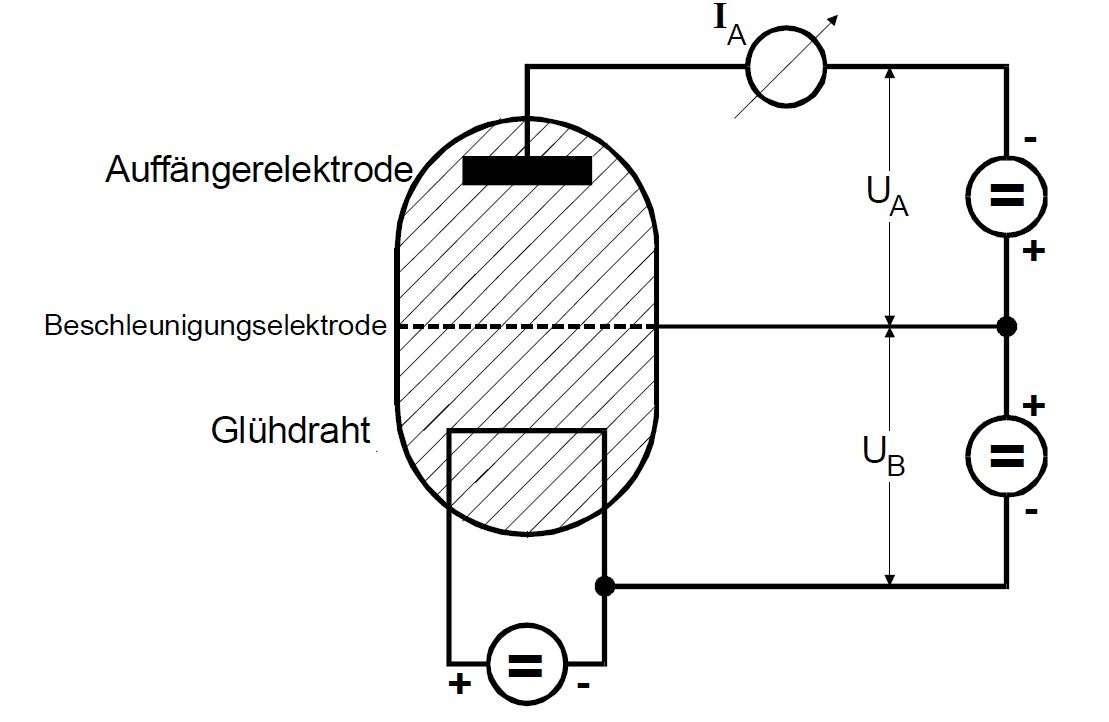
\includegraphics[scale=0.3]{picaufbaugrob.jpg}
		\caption{Prinzipieller Aufbau des Franck-Hertz-Versuches [1]}
		\label{picaufbaugrob}
		\end{center}	
	\end{figure} 	\begin{figure}[h]
		\begin{center}
		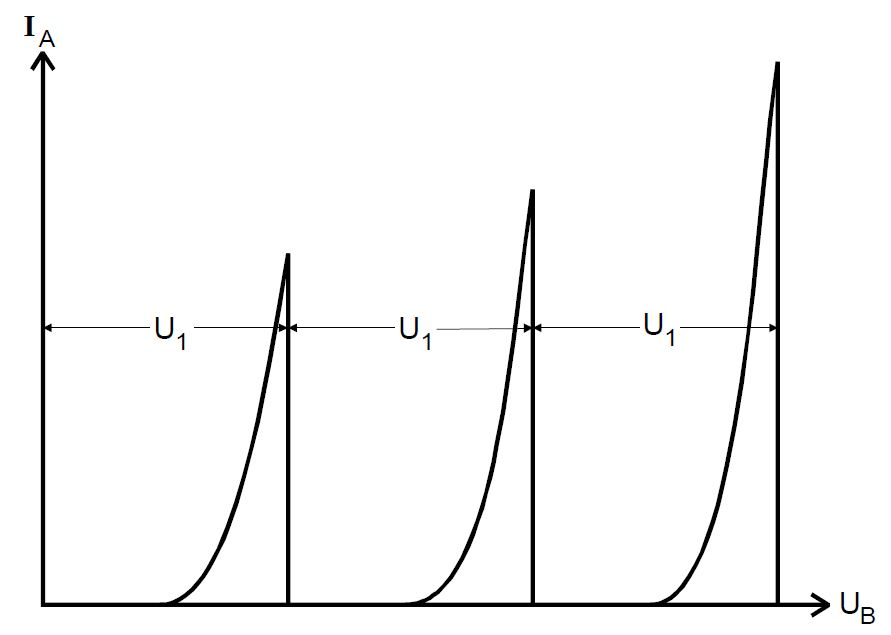
\includegraphics[scale=0.3]{picfhkurvet.jpg}
		\caption{Idealisierter Kurvenverlauf eines Franck-Hertz-Versuches [1]}
		\label{picfhkurvet}
		\end{center}	
	\end{figure}
Der grundsätzliche Aufbau einer Messanordnung zum Franck-Hertz-Versuch ist in Abbildung \ref{picaufbaugrob}
dargestellt. 
In der evakuierten Röhre befindet sich ein wenig Quecksilber, welches temperaturabhängig verdampft.
An dem einen Ende der Röhre befindet sich ein Glüdraht, aus dem beim Erhitzen Elektronen austreten, 
in der Mitte liegt eine netzförmige Beschleunigungselektrode, welche dem Glühdraht gegnüber eine
Beschleunigungsspannung aufbaut, und an dem anderen Ende befindet sich eine Auffängerelektrode,
welche eine Gegenspannung gegenüber der Beschleunigungselektrode besitzt und abhängig von der
eintreffenden Anzahl von Elektronen einen Auffängerstrom registriert.
Bei einem temperaturabhängigem Gleichgewichtsdampfdruck $p_{\text{sät}}$ von Hg-Dampf 
werden Elektronen aus dem Glühdraht emittiert und mit einer Beschleunigungsspannung $U_B$ zu der
Beschleunigungselektrode hin beschleunigt. Schließlich werden sie nach Durchlaufen des 
Gegenfeldes mit der Abbremsspannung $U_A$ an der Auffängerelektrode als Auffängerstrom $I_A$
gemessen. Um aber überhaupt das Gegenfeld durchlaufen zu können, muss die Geschwindigkeitskomponente
des Elektrons in Feldrichtung, $v_Z$, die Ungleichung
\begin{align}
\frac{m_{e^-}}{2} v_Z^2 &\geq e_0 U_A 
\end{align}
mit $m_{e^-}$ als die Ruhemasse des Elektrons, $e_0$ als die Elementarladung, erfüllen \cite{anleitung}.\\
Eine beispielhafte theoretische Kurve des Auffängerstroms in Abhängigkeit von $U_B$ ist in
Abbildung \ref{picfhkurvet} dargestellt. Sobald die Elektronen genug Energie besitzen um die 
Abbremsspannung überwinden können, steigt $I_A$ kotinuierlich an. Sobald die Elektronen jedoch
genug Energie besitzen um inelastische Stöße durchzuführen, sinkt $I_A$ stark ab, da die Elektronen
fast alle Energie an die Hg-Atome abgegeben haben (vgl. Gl. (\ref{eqanreg})). Wird $U_B$ nun weiter
erhöht, wiederholt sich der Vorgang mit dem Unterschied, dass es nun zu mehreren inelastischen Stößen 
kommen kann. Der Abstand $U_1$ hängt dabei über Gleichung (\ref{equ1}) mit dem ersten Anregungspotential 
zusammen. Fällt das Hg-Atom nun wieder aus diesem zurück, wird Licht mit der Frequenz $f$ nach Gleichung
(\ref{eqlicht}) emittiert \cite {anleitung}.
\begin{align}
U_1=\frac{1}{e_0}(E_1-E_0) \label{equ1} \\
h\cdot f &= E_1-E_0 \text{ , $h$: Planksches Wirkungsquantum} \label{eqlicht}
\end{align}
Desweitern lässt sich mit dieser Versuchsanordnung bei ausreichender Abbremsspannung zum Abhalten
der Elektronen von der Auffängerelektrode und zur Messung der Ionen, die 
Ionisierungsenergie von Hg bestimmen. Ebenfalls kann die differentielle Energieverteilung der Elektronen,
welche aus dem Auffängerstrom, beziehungsweise von $U_A$ abhängt, aufgezeichnet werden.
Um die Anzahl der Elektronen der Energie zwischen $E_Z$ und $E_Z + \Delta E_Z$ zu bestimmen, wird
die Differenz der jeweiligen Ströme bestimmt, wo gilt:
\begin{align}
E_Z&=e_0 U_A \\
E_Z + \Delta E_Z &= e_0 (U_A + \Delta U_A) \label{eqbla}
\end{align}
\subsection{Störeffekte}
 Die reale Messkurve des Versuches ist aufgrund verschiedener Störfaktoren im Vergleich zu Abbildung
 \ref{picfhkurvet} verschoben, verbreitert und abgeflacht. \\
 
 Ein Störfaktor ist das auftretende Kontaktpotential zwischen dem Glühdraht niedriger Austrittsarbeit
$\Phi_G$ 
 und der Beschleunigungselektrode höherer Austrittsarbeit $\Phi_B$. 
 Dadurch kommt es zu einer Verschiebung um das Kontaktpotential $K$
 der Kurve, da $U_B$ von der effektiven Beschleunigungsspannung abweicht.
 \begin{align}
 U_{B, \text{eff}}&=U_B - \frac{1}{e_0} (\Phi_B - \Phi_G) \\
 K&:=\frac{1}{e_0}(\Phi_B - \Phi_G)
 \end{align}
\\
Ein weiterer Störeinfluss ist das durch die Fermi-Dirac-Verteilung der Energie der Elektronen des 
Glühdrahtes auftretende Energieverteilung der Elektronen. Dadurch sind die Elektronen nicht 
monoernergetisch, sodass die Kurve abgeflacht und verbreitert wird. Ebenfalls störend sind die 
elastischen Stöße der Elektronen mit den Hg-Atomen im Bereich der Abbremsspannung, denn dadurch ändert 
sich die Richtung und damit die Reichweite der Elektronen im Gegenfeld.\\
Störend wirkt außerdem ein nicht idealer Dampfdruck des Hg-Dampfes, welcher von der Temperatur $T$ abhängt.
Ist der Druck zu gering, kommt es
nicht immer zu den erwünschten Wechselwirkungen, ist der Druck zu hoch, gibt es zu viele unerwünschte 
inelastische Stöße. Die mittlere freie Weglänge der Atome, $\overline w$, muss klein gegenüber dem
Abstand $a$ zwischen Kathode und der Beschleunigungselektrode sein.
\begin{align}
\overline w &=\frac{2,9\cdot 10^{-8}}{p_{\text{sät}}} \label{eqwstrich}\\
p_{\text{sät}}(T)&=5,5 \cdot 10^{4} \cdot exp(-6876/T) \label{eqdruck}
\end{align} 
